%%%%%%%%%%%%%%%%%%%%%%%%%%%%%%%%%%%%%%%%%%%%%%
%                insertmeeting
% 1) Title (something creative & funny?)
% 2) Date (MM/DD/YYYY)
% 3) Location (ex. Hagerty High School)
% 4) People/Committees Present 
% 5) Picture 
% 6) Start Time & Stop Time (ex. 12:30AM to 4:30PM)
%%%%%%%%%%%%%%%%%%%%%%%%%%%%%%%%%%%%%%%%%%%%%%
\insertmeeting 
	{New Chassis Design} 
	{10/10/21}
	{Hagerty High School}
	{Jensen, Nathan, Ritam, Samantha}
	{Images/RobotPics/robot.jpg}
	{12:30 - 4:30}
	
\subsection*{Hardware}
\noindent\hfil\rule{\textwidth}{.4pt}\hfil
\subsubsection*{Goals}
\begin{itemize}
    \item Build new car drive chassis  

\end{itemize} 

\noindent\hfil\rule{\textwidth}{.4pt}\hfil

\subsubsection*{Accomplishments}
n Lab, where our mentor, Mr. Harper, works. The lab has lots of important resources like laser cutters and 3D printers that are key to how our hardware team functions, so it felt good to be back in the lab after a year-long hiatus. To start building our car drivetrain, we looked at our small tank drivetrain and tried to find extrusions of a similar length. Once we found them we began screwing all of the parts together into a rectangle. To attach our motors and wheels, we started laser cutting our motor mounts and gear brackets that we designed at the last meeting. While cutting these parts, we remembered that we currently don’t have a good place to put the rev hub and battery so we measured the part of the drivetrain we had already built and made a quick CAD design that we could cut out and screw to our chassis (Figure \ref{fig:pic1}). Being able to make very quick design changes and improvements like this one is a big reason why we love working at UCF. Because everything is so available and easy to use with the help of our mentor, we can get into a good flow while working in the innovation lab. 
With all of the pieces cut out, we started screwing them onto the rectangle we had made earlier (Figure \ref{fig:pic2}). Our wheels are driven by gears connected to two HD Hex 20:1 motors. The decision to use REV extrusions, gears, and REV HD Hex motors was driven by their ease of construction, not by their mechanical advantages. Once we test out this design and ensure that using it is even a possibility, we Follow the engineering design process to make improvements. Right now we built the drivetrain to be simple, but in the season overall, we always work hard to make our robots high quality and well designed. One design change that we are already talking about is switching from gears to either belts or chains, both of which are better options for the job. One crazy idea that we came up with for the main structure of the drivetrain is to 3D print the whole structure. Because we are making such a small drivetrain this year, we noticed that we could print the entire drivetrain inside the Fortus 450 at UCF out of polycarbonate, a very strong type of plastic. With all of these ideas in mind, we still needed to complete this iteration of the drivetrain before moving on to new ideas. 


\begin{figure}[ht]
\centering
\begin{minipage}[b]{.50\textwidth}
  \centering
  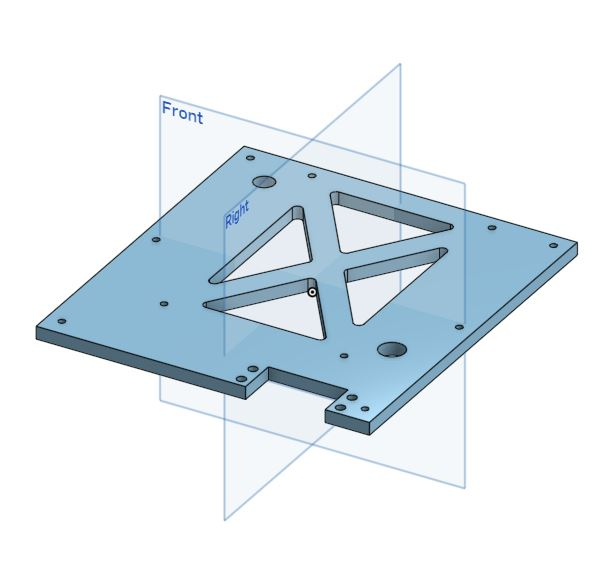
\includegraphics[width=0.8\textwidth]{Meetings/October/10-10-21/10-10-2021_Hardware_Figure1 - Nathan Forrer.JPG}
  \caption{Our modified RevHub and battery mount.}
  \label{fig:pic1}
\end{minipage}%
\hfill%
\begin{minipage}[b]{.50\textwidth}
  \centering
  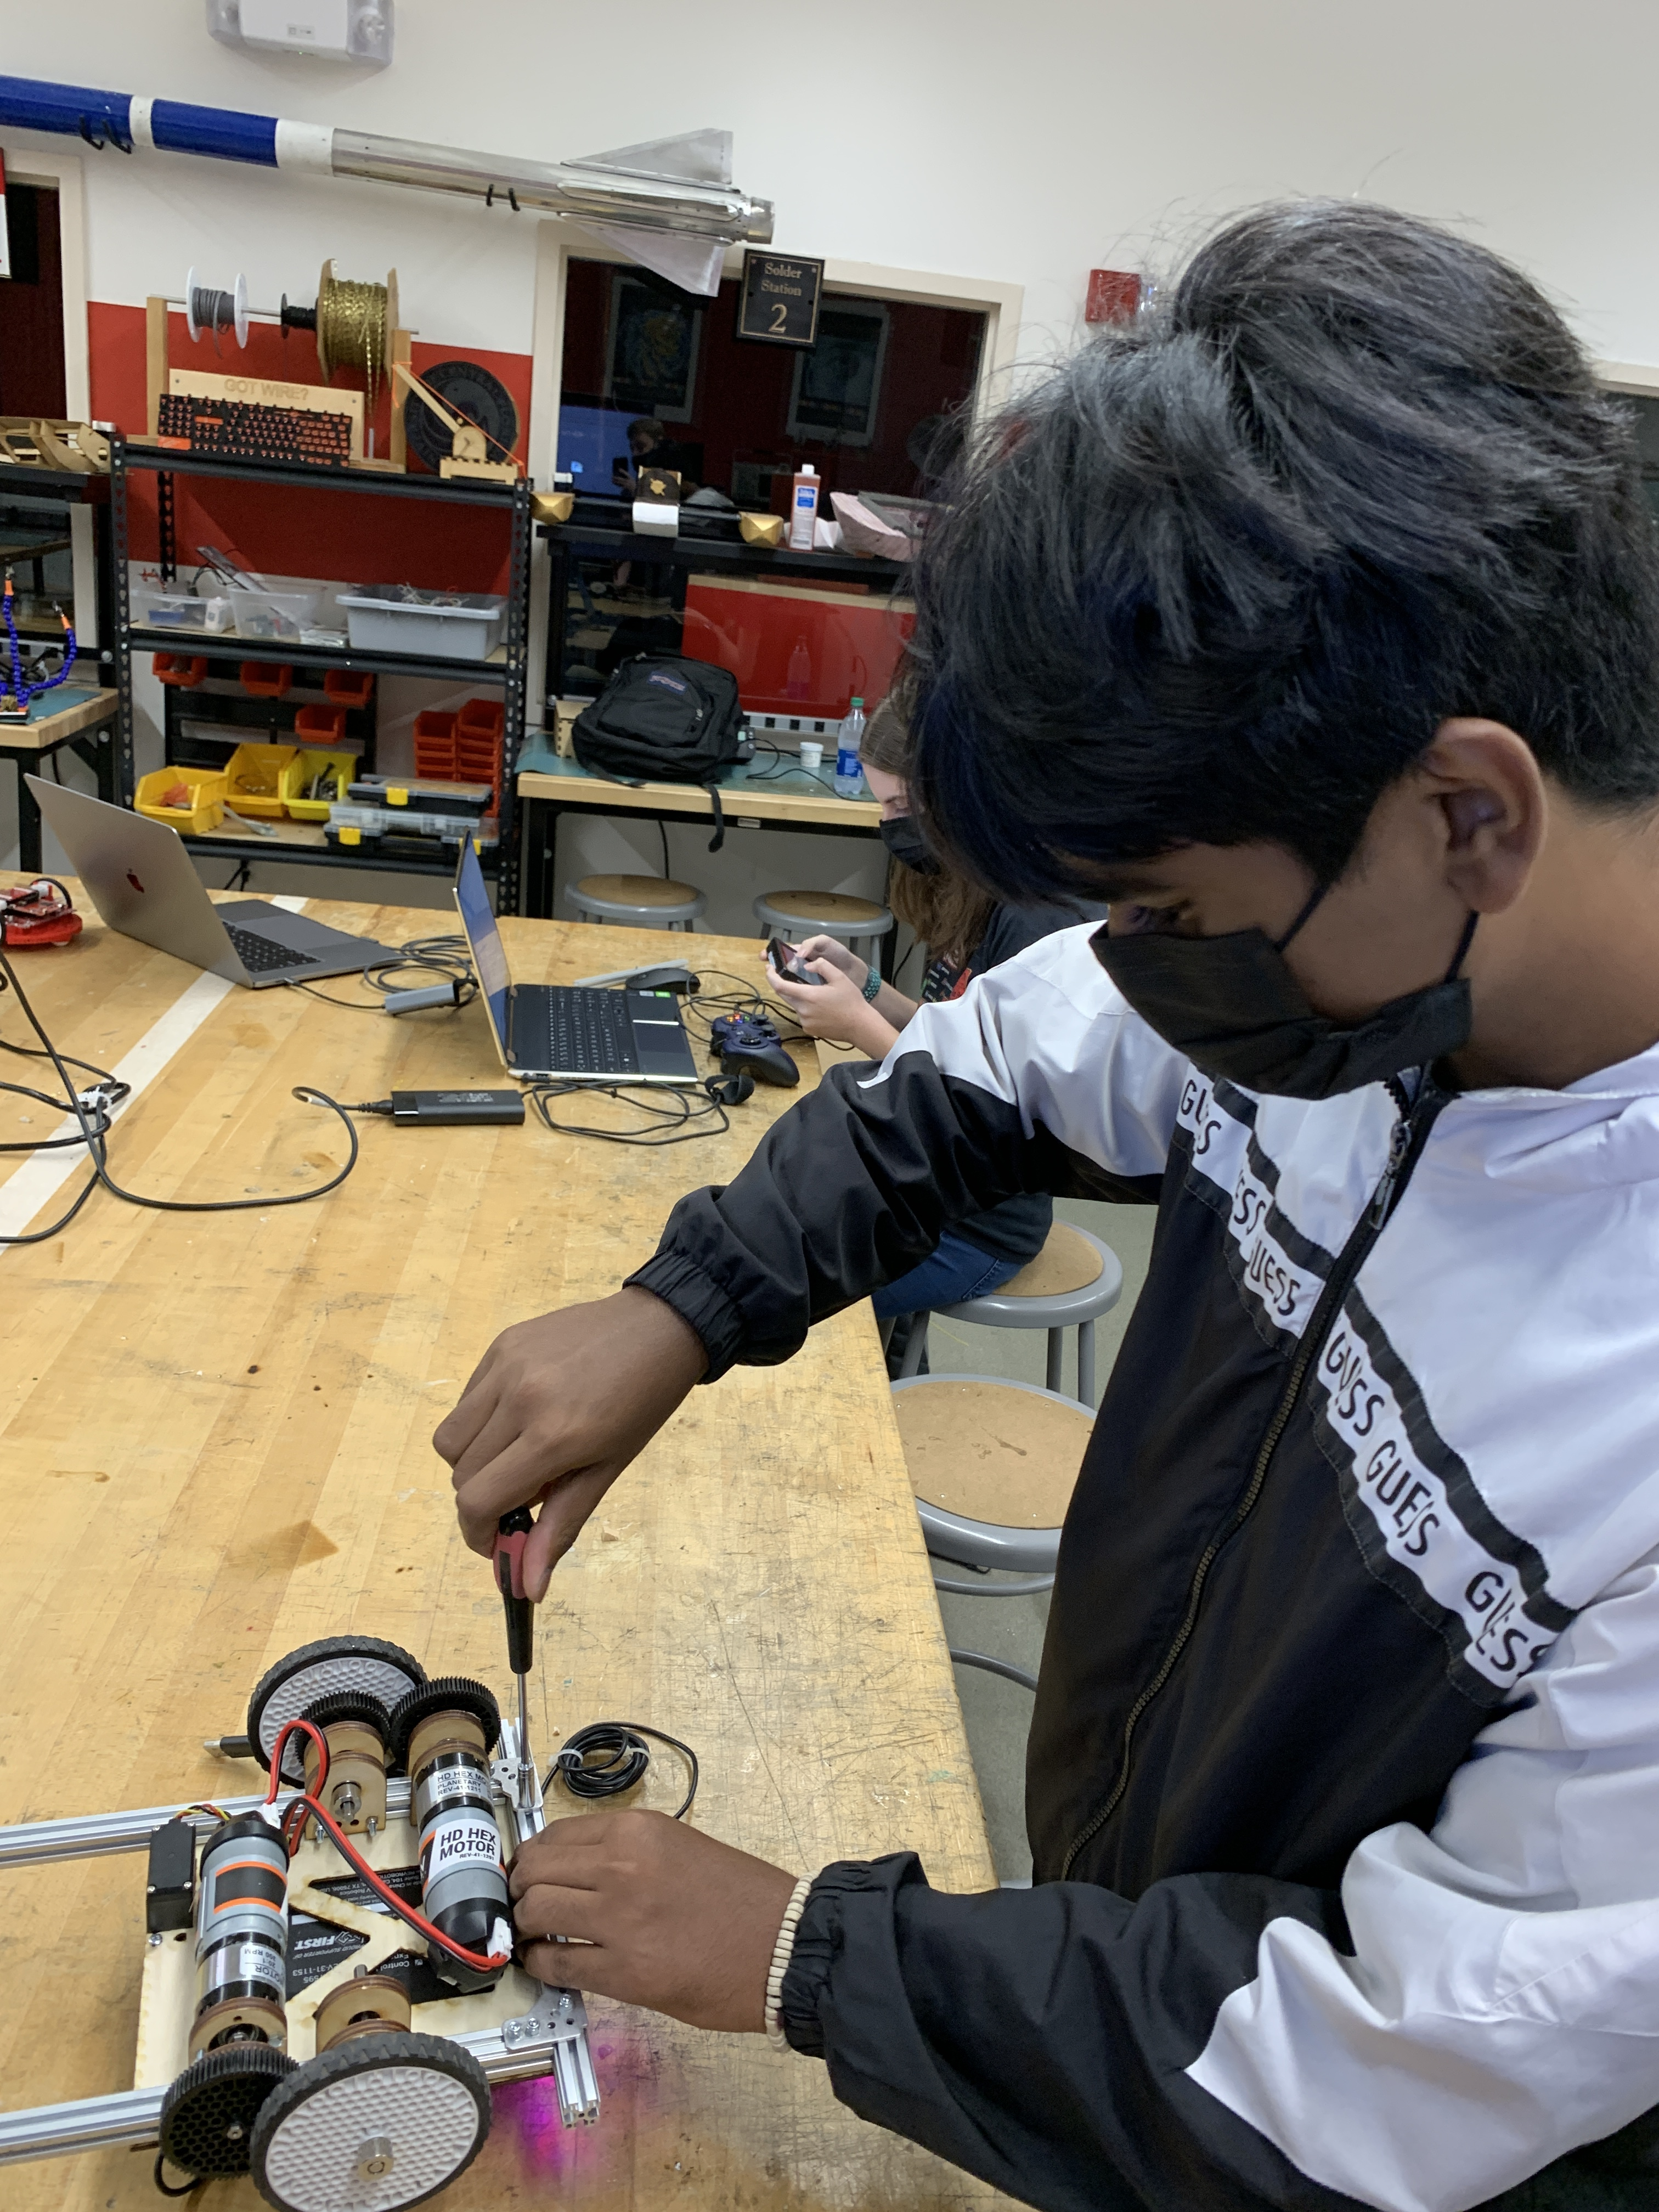
\includegraphics[width=0.8\textwidth]{Meetings/October/10-10-21/10-10-2021_Hardware_Figure2 - Nathan Forrer.JPG}
  \caption{Ritam hard at work on our tricycle drive prototype.}
  \label{fig:pic2}
\end{minipage}
\end{figure}







